\chapter{RESULTADOS E DISCUSSÃO }

\section{Alcance da amostra}



Para o desenvolvimento do programa foi alcançado 26 equipes apresentando ao todo 118 alunos oriundos dos cursos do centro de agrárias e mais outras áreas: \textit{Artes Visuais}, \textit{Administração}, \textit{Design Gráfico}, \textit{Engenharia Química}, \textit{Engenharia de Produção}, \textit{Marketing e Ecologia}. 



Os dados coletados revelam que, nas 63 respostas válidas que compõem a amostra, a divisão de gênero está equilibrada, sendo que 33 eram homens e 30 mulheres. Em relação à faixa etária quando realizaram o programa de mobilidade acadêmica, 67\% dos estudantes possuíam entre 19 e 22 anos e 30\% apresentaram a intervalo de idades entre 23 e 26 anos.



\begin{table}[!htb]
\caption{\textbf{Faixa etária dos alunos inscritos no programa}}
\label{tab:tabela_4}
\begin{tabular}{clccc}
\hline \hline
{\color[HTML]{000000} \textbf{Dados}} & {\color[HTML]{000000} \textbf{Faixa etária}} & \multicolumn{3}{c}{{\color[HTML]{000000} \textbf{Inscritos}}} \\ \cline{1-5}
{\color[HTML]{000000} } & {\color[HTML]{000000} } & \multicolumn{1}{l}{{\color[HTML]{000000} \textbf{Frequência (\%)}}} & \multicolumn{1}{l}{{\color[HTML]{000000} \textbf{Porcentagem (\%)}}} & \multicolumn{1}{l}{{\color[HTML]{000000} \textbf{Porcentagem válida (\%)}}} \\
{\color[HTML]{000000} } & {\color[HTML]{000000} \textbf{Menor que 20}} & {\color[HTML]{000000} 89} & {\color[HTML]{000000} 75,4} & {\color[HTML]{000000} 77,4}\\[8pt]
\multirow{-3}{*}{{\color[HTML]{000000} \textbf{}}} & {\color[HTML]{000000} \textbf{De 21 a 25}} & {\color[HTML]{000000} 19} & {\color[HTML]{000000} 16,1} & {\color[HTML]{000000} 16,5} \\[8pt]
\multicolumn{1}{l}{{\color[HTML]{000000} \textbf{Válidos}}} & {\color[HTML]{000000} \textbf{Maior que 25}} & {\color[HTML]{000000} 7} & {\color[HTML]{000000} 5,9} & {\color[HTML]{000000} 6,1}\\[8pt]
\multicolumn{1}{l}{{\color[HTML]{000000} \textbf{}}} & {\color[HTML]{000000} \textbf{Total}} & {\color[HTML]{000000} 115} & {\color[HTML]{000000} 97,5} & {\color[HTML]{000000} } \\[8pt]\hline
\multicolumn{1}{l}{{\color[HTML]{000000} \textbf{Omissos}}} & {\color[HTML]{000000} \textbf{Não informou}} & {\color[HTML]{000000} 3} & {\color[HTML]{000000} 2,5} & {\color[HTML]{000000} } \\[8pt] \hline
\multicolumn{2}{c}{{\color[HTML]{000000} \textbf{TOTAL GERAL}}} & {\color[HTML]{000000} 118} & {\color[HTML]{000000} } & {\color[HTML]{000000} } \\ \hline\hline
\end{tabular}
\fonte{Autoria própria}
\end{table}

O curso que mais apresentou inscrições dos alunos foi o de Engenharia Agronômica, representando 47,32\% deste total, enquanto os cursos de Engenharia Agrícola, Zootecnia, Engenharia de Pesca e Engenharia Florestal tiveram participações consideravelmente menores, com apenas 11,61\%, 19,64\%, 4,46\% e 6,25\% dos estudantes inscritos, respectivamente, já o curso de Medicina veterinária não apresentou alunos inscritos. Na figura  \ref{figura_10} é possível observar a quantidade de alunos inscritos e seus respectivos cursos.

\begin{figure}[!htb]
\centering
\caption{\textbf{Porcentagem de alunos inscritos no programa por curso}}
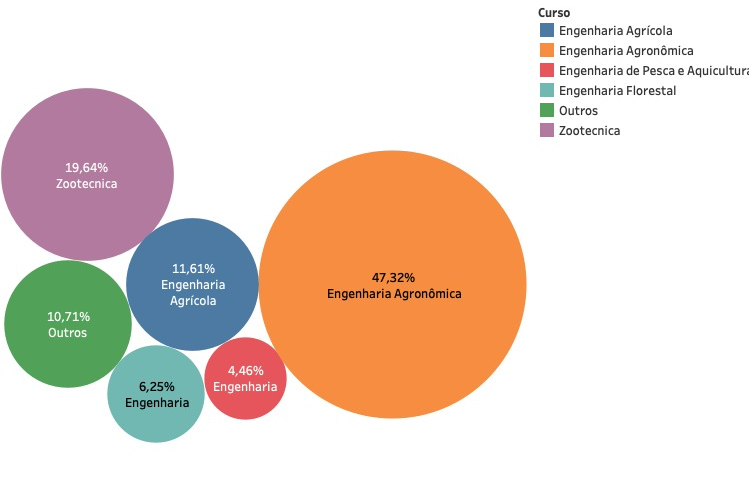
\includegraphics[scale=0.4]{Imagens/inscritos.png}
\fonte{Autoria própria}
\label{figura_10}
\end{figure}

\newpage

\section{Tratamento dos grupos de itens: Autoeficácia, Intenção empreendedora, Apoio Familiar}

O método de rotação Varimax com normalização de Kaiser\footnotemark[1] apresentou 3 componentes principais para esta pesquisa, aglutinando as questões na ordem apresentada na tabela \ref{tabela_3}:


\begin{center}
 %\large

\begin{longtable}{p{6cm} c c c }

\caption{\textbf{Estrutura fatorial da medida de intenção empreendedora}}

\label{tabela_3} \\ \hline\hline

\multicolumn{1}{p{6cm}}{} & \multicolumn{3}{c}{\textbf{Fatores}}\\ 
 \multicolumn{1}{c}{\textbf{Itens}} & \multicolumn{3}{c}{\hrulefill}\\ 

 \multicolumn{1}{c}{} 
 &\multicolumn{1}{p{1.5cm}}{\textbf{Autoeficácia}} & \multicolumn{1}{p{1.5cm}}{\textbf{Intenção}} &\multicolumn{1}{p{1.5cm}}{\textbf{Família}}  
\\ \hline 

\endfirsthead


\multicolumn{4}{l}{{{\bfseries \tablename \ \thetable{} -\ \textbf{Estrutura fatorial da medida de intenção empreendedora}}}}\\
\multicolumn{4}{r}{\bfseries \textbf{(continuação)}}\\

\hline \multicolumn{1}{p{6cm}}{\textbf{Questões}} &\multicolumn{1}{c}{\textbf{Autoeficácia}} & \multicolumn{1}{c}{\textbf{Intenção}} &\multicolumn{1}{c}{\textbf{Família}}  
\\ \hline 

\endhead

\hline \multicolumn{4}{r}{\textbf{(Continua)}} \\ \hline


\endfoot
\hline \multicolumn{4}{r}{\textbf{(Conclusão)}} \\ \hline
\hline \hline

\endlastfoot


Estabelecer e atingir metas e objetivos
 &  0,776 & & \\\\
 
Gerar novas ideias
 &  0,785 & & \\\\
 
Desenvolver novos produtos
 &  0,682 & & \\\\
 
Fazer análises financeiras
 &  0,739 & & \\\\
 
Reduzir riscos e incertezas
 &  0,746 & & \\\\
 
Assumir riscos calculados
 &   0,756 & & \\\\
 
 Tomar decisões em situações de risco
 &   0,637 & & \\\\
 
Administrar o tempo estabelecendo metas
 &   0,650 & & \\\\
 
Responsabilizar-me por ideias e decisões
 & 0,465
& \textbf{0,577} &  \\\\

Começar minha própria empresa
 & 0,456 & \textbf{0,592}  & \\\\
 
Para mim, ser um empreendedor implica em mais vantagens do que desvantagens
 &  & 0,894  & \\\\
 
Uma carreira como empreendedor é atrativa
 &  & 0,817  & \\\\
 
Se tivesse a oportunidade e os recursos, eu me tornaria um empreendedor
 &  & 0,892 & \\\\
 
Ser um empreendedor traria grande satisfação
 &  & 0,905 & \\\\
 
O capital oferecido por minha família e empréstimo em condições flexíveis são facilitadas
 &  & & 0,905 \\\\
 
Minha família me fornece contatos com pessoas que podem me ajudar na carreira de empreendedor
 &  & & 0,779 \\\\
 
Minha família me apresenta pessoas de sua rede de relação de negócios
 &  & & 0,621 \\\\
 
Minha família me transmite conhecimentos ligados ao meu setor de atividade
 &  & & 0,806 \\\\
 
Meus pais / minha família são meus mentores ou \textit{coachs} nas minhas atividades de empreendedor
 &  & & 0,820 \\\\
 
Minha família me fornece locais/ infraestrutura para minhas atividades de empreendedor.
 &  & & 0,682 \\\\
 
Meus pais ou família me concedem acesso a uma rede de distribuição para minha empresa.
 &  & & 0,722 \\\\
 
 Pensando em todos os possíveis recursos que minha família me fornece, sou completamente independente dela para decidir como alocá-los e usá-los.
 &  & & 0,661 \\\\
 
Minha família me empresta capital que  tenho que pagar regularmente a eles com juros		
 &  & & 0,692 \\\\
 
Minha família me empresta capital sem a necessidade de juros e que pode ser perdido se o negócio falir
 & & & 0,512 \\\\ \hline 
 
\end{longtable}
\fonte{Autoria própria}
\end{center}
\footnotetext[1]{Método de Extração: Análise de Componente Principal.\\Método de Rotação: Varimax com Normalização de Kaiser.}



\begin{table}[!htb]
 \label{tabela_4}
 \centering
\caption{\textbf{Variância total explicada}}
 \\ \hline\hline
\begin{tabular}{c c c c }
\multicolumn{1}{p{6cm}}{} & \multicolumn{3}{c}{\textbf{Fatores}}\\ 
 \multicolumn{1}{c}{\textbf{Itens}} & \multicolumn{3}{c}{\hrulefill}\\ 

 \multicolumn{1}{c}{} 
 &\multicolumn{1}{c}{\textbf{Autoeficácia}} & \multicolumn{1}{c}{\textbf{Intenção}} &\multicolumn{1}{c}{\textbf{Família}}  
\\\\ \hline 

 Somas de rotação de carregamentos ao quadrado (n)
 & 5,526 & 5,014 & 4,604 \\\\
 Variância explicada (\%)
 & 19,05 & 17,30 &15,87\\\\
 Variância cumulativa (\%)
 & 19,05\% & 36,34\% &52\% \\\hline \hline 
 
\end{tabular}
\fonte{Adaptado de \cite{lima_sauglobal_2017}}.
\end{table}



As questões: \textbf{"Para mim sem empresa não e autônomo"}, \textbf{"Eu já sou meu próprio patrão na empresa que eu fundei"} e \textbf{"Tenho precisão consistente do que empreender e datas para os passos da fundação"}, foram eliminadas da pesquisa, pois foi adotado a supressão de coeficientes que apresentaram valores absolutos a baixo de 0,40, Já as questões: \textbf{Responsabilizar-me por ideias e decisões} e \textbf{Começar minha própria empresa}, apresentaram valores satisfatórios tanto para dimensão Autoeficácia quanto para dimensão intenção empreendedora, porem foi considerado o valor de coeficiente mais alto.


\section{Resultados do estudo}

Os resultados encontram-se divididos em seções, atendendo aos objetivos do estudo. Inicialmente  serão  apresentadas  descrições  que  caracterizam  os  dois  grupos  (pré-programa  e pós-programa) em relação às variáveis e as comparações entre os grupos.

\subsection{Áreas e cadeias produtivas}


A fase inicial do programa foram alcançadas 27 propostas de protótipos e/ou negócios na área rural com foco na agricultura sustentável. Na figura \ref{figura_11} é possível verificar as áreas e cadeias produtivas prioritárias escolhidas.


\begin{figure}[!H]
\centering
\caption{\textbf{Áreas e potenciais propostas de negócios escritos}}
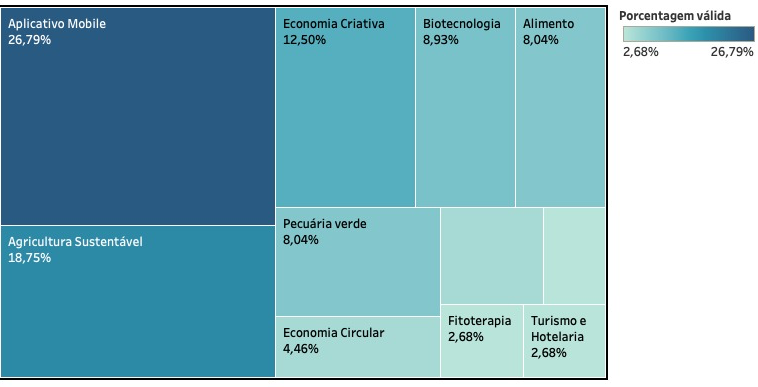
\includegraphics[scale=0.5]{Imagens/propostas_negocios.png}
\fonte{Autoria própria}
\label{figura_11}
\end{figure}

